\documentclass[oneside,a4paper,spanish,links]{amca}
%
\usepackage{graphicx}
\usepackage{amsmath,amsfonts}
\usepackage[utf8]{inputenc}
%
\title{SIMULACIÓN DE TRANSITORIOS CON SOLVER PIMPLEFOAM}
%
\englishtitle{TRANSIENT SIMULATION WITH PIMPLEFOAM SOLVER}

\author[a]{Guillermo Rolle}
%\author[b]{Segundo B. Autor}
%\author[b]{Tercer C. Autor}
%\author[a]{Cuarto D. Autor}
%
%\affil[a]{Grupo de Mecánica Computacional, Universidad Nacional de
%Villa Carolina, Los Alerces 3492, 4200~Villa Carolina, Argentina,
%gmc@uncarolina.edu.ar, \url{http://www.uncarolina.edu.ar/gmc}}
%
%\affil[b]{Grupo de Ingeniería Aplicada, Universidad Nacional de La
%Meseta, Los Cipreses 3493, 4201~La Meseta, Argentina,
%gia@unmeseta.edu.ar, \url{http://www.unmeseta.edu.ar/gia}}

%% NOTA: SI TODOS LOS AUTORES TIENEN LA MISMA AFILICACION
%% USE EL MACRO `\voidaffil' PARA EL CODIGO DE AFILICACION.
%% Ejemplo:
%% \author[\voidaffil]{Primer A. Autor}
%% \author[\voidaffil]{Segundo B. Autor}
%% \author[\voidaffil]{Tercer C. Autor}
%% \author[\voidaffil]{Cuarto D. Autor}
%% %
%% \affil[\voidaffil]{Grupo de Mecánica Computacional,
%% Universidad Nacional de Villa Carolina,
%% Los Alerces 3492, 4200 Villa Carolina, Argentina,
%% gmc@uncarolina.edu.ar, http://www.uncarolina.edu.ar/gmc}

\begin{document}
\vspace{3cm}

\maketitle

%% To set PDF METADATA: uncomment and replace fields in
%% UPPERCASE with appropriate values.
%%
%% \hypersetup{
%%   pdfauthor={AUTHORS},
%%   pdfkeywords={KEYWORDS},
%%   pdftitle={TITLE}
%% }
%%
%% For instance
%% \hypersetup{
%%   pdfauthor={Sponge B. and Star P.},
%%   pdfkeywords={multiphase flow, air-liquid mixtures},
%%   pdftitle={A new model for multi-phase flow}
%% }
%%
%% NOTE: To set the metadata is recommended but not absolutely
%% neccesary.
%% This was done before with the \pdfinfo command,
%% but according to this post:
%% http://de.nntp2http.com/comp/text/tex/2008/12/5358fd061de9703a781885a5dcf98364.html
%% if `hyperref' is used, then you must use \hypersetup{} not \pdfinfo{}

\begin{keywords}
CFD, OpenFOAM, pimpleFoam 
\end{keywords}

\begin{abstract}
Este documento provee una guía para realizar una simulación de estado transitorio en OpenFOAM utilizando el solver pimpleFoam. La malla es importada de un informe anterior al igual que las condiciones de contorno e iniciales. El informe provee también una breve explicación sobre técnicas de post-proceso y conclusiones sobre el método implementado.
\linebreak
%
\linebreak
%
\textbf{Keywords:} CFD, OpenFOAM, pimpleFoam\\
%
\linebreak
%
\textbf{Abstract.}
This document provides a guide to perform a transient state simulation in OpenFOAM using the pimpleFoam solver. Mesh is imported from a previous report like boundary and initial conditions. The report also provides a brief explanation of post-processing techniques and conclusions about the implemented method. 

%\\
%\\
%\textbf{Agradecimientos:} Los autores agradecen... (no más de 2 líneas)
% LOS AGRADECIMIENTOS EN LA PRIMERA PAGINA SE PERMITEN SOLO PARA
% PRESENTACIONES DE RESUMENES (NO PARA ARTICULOS COMPLETOS)
\end{abstract}

\section{INTRODUCCIÓN}
En el \href{https://github.com/guillerolle/informes_cfd/blob/master/Informe03.pdf}{informe anterior} se hicieron simulaciones en 3D sobre el mezclador de agroquímicos. Los campos de velocidad y presión fueron obtenidos con un solver estacionario. Se había comprobado que el solver no era capaz de reducir los residuales al valor requerido por no poder obtenerse una solución estacionaria. En este informe se simula el mismo caso pero con el solver transitorio \href{https://www.openfoam.com/documentation/guides/latest/doc/guide-applications-solvers-incompressible-pimpleFoam.html}{pimpleFoam}. Se usa una copia de la malla previa y el informe se basará exclusivamente en las modificaciones del caso para ejecutar el nuevo solver. 

\begin{figure*}[htb]
	%%\centerline{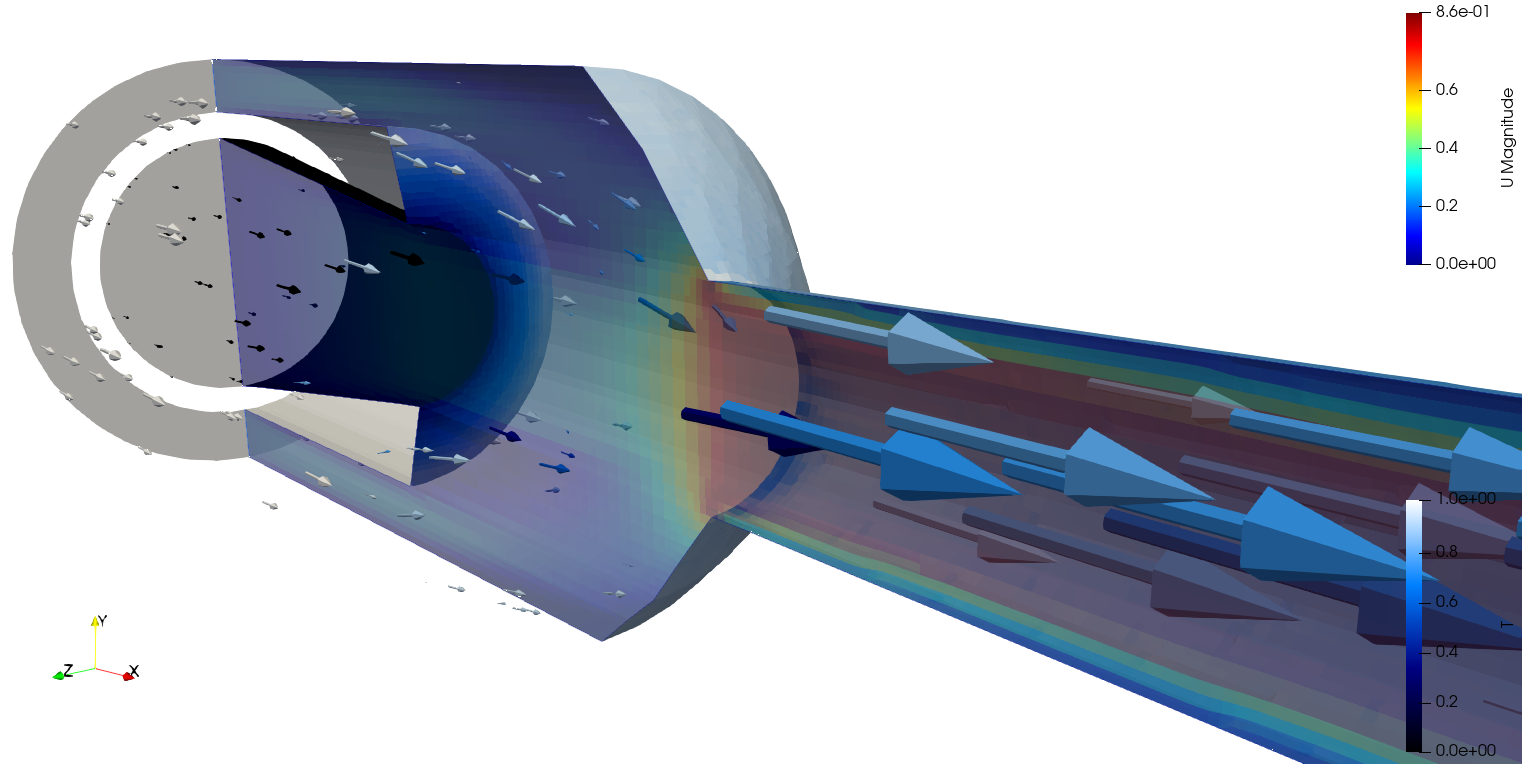
\includegraphics[width=0.8\textwidth]{Figuras/05_GLYPH.png}} 
	\caption{Caso 3D en cuestión} \label{fg:intro}
\end{figure*}

Este informe es parte de la \href{https://github.com/guillerolle/informes_cfd}{serie de informes} basados en un mezclador de agroquímicos en línea. El material correspondiente para este caso se encuentra en el \href{https://github.com/guillerolle/casos_cfd}{repositorio online}.

\section{PREPARACIÓN DEL CASO}
Usamos el \href{https://github.com/guillerolle/casos_cfd/tree/master/03/case}{caso 3D anterior} como base para preparar el nuevo caso. Copiamos además el \href{https://github.com/guillerolle/casos_cfd/tree/master/03/meshCase}{meshCase} para generar la malla. Notar que no modificaremos los parámetros de mallado pero aprovecharemos el script \href{https://github.com/guillerolle/casos_cfd/tree/master/03/case/Allrun}{Allrun} que requiere de la existencia de este caso.

No son muchas las modificaciones que hay que hacer para pasar de una simulación con \texttt{simpleFoam} a una con \texttt{pimpleFoam}. 

Primero, en el archivo \href{https://github.com/guillerolle/casos_cfd/tree/master/04/case/system/controlDict}{controlDict} debemos llenar el campo \texttt{application} con \texttt{pimpleFoam}. Además, en el solver estacionario el campo \texttt{deltaT} representa el paso en la numeración de iteraciones y no representa más que un número de iteración. En un solver transitorio en cambio, sí es importante ya que representa el paso de tiempo entre una iteración y la siguiente. Lo mismo aplica para el campo \texttt{endTime}. Para la simulación de transitorio simularemos un tiempo total de 2 segundos con paso de tiempo de 1ms como se ve en la figura \ref{fg:controlDict}. Por último, aumentamos la frecuencia de escritura para poder analizar mejor las variaciones en el tiempo.

\begin{figure*}[htb]
	\centerline{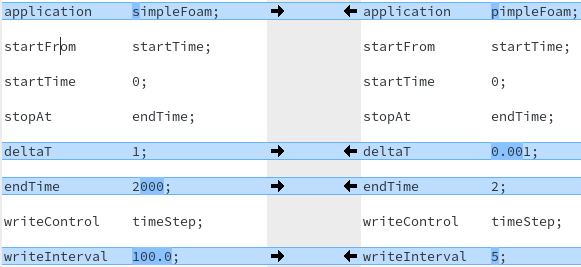
\includegraphics[width=0.8\textwidth]{Figuras/02_controlDict_1.png}}
	\caption{cambios en controlDict: caso estacionario (izquierda) vs caso transitorio (derecha)} \label{fg:controlDict}
\end{figure*}

En el archivo \href{https://github.com/guillerolle/casos_cfd/tree/master/04/case/system/fvSchemes}{fvSchemes} modificamos el campo \texttt{ddtSchemes} y agregamos una línea a \texttt{gradSchemes}. Los cambios se muestran en la figura \ref{fg:fvSchemes}.

\begin{figure*}[htb]
	\centerline{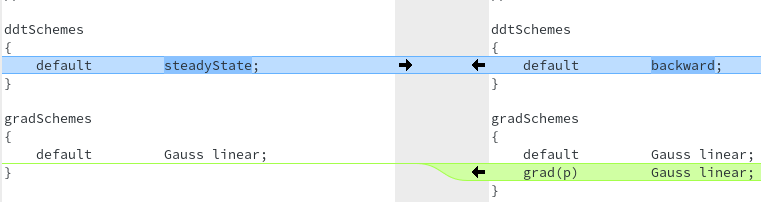
\includegraphics[width=0.8\textwidth]{Figuras/02_fvSchemes_1.png}} 
	\caption{cambios en fvSchemes: caso estacionario (izquierda) vs caso transitorio (derecha)} \label{fg:fvSchemes}
\end{figure*}

\newpage

Por último, modificamos las tolerancias de los solvers para \texttt{p} y \texttt{U} en el archivo \href{https://github.com/guillerolle/casos_cfd/tree/master/04/case/system/fvSolution}{fvSolution}. Además, agregamos los modificadores para el campo \texttt{PIMPLE}. los cambios se muestran en la figura \ref{fg:fvSolution}

\begin{figure*}[htb]
	\centerline{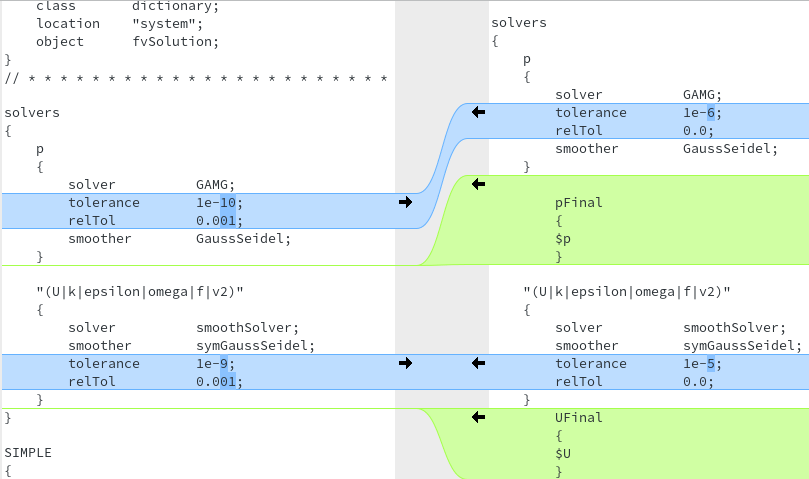
\includegraphics[width=0.8\textwidth]{Figuras/02_fvSolution_1.png}} 
	\centerline{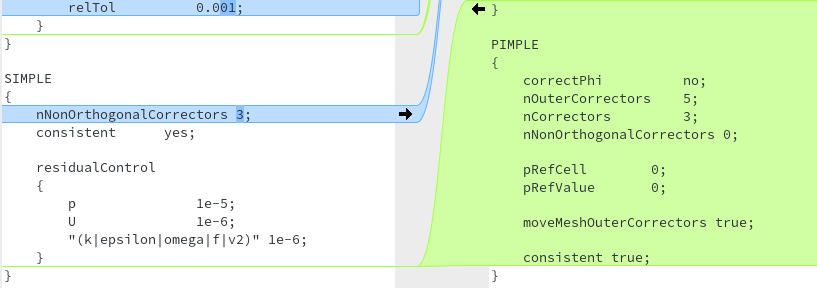
\includegraphics[width=0.8\textwidth]{Figuras/02_fvSolution_2.png}}
	\caption{cambios en fvSolution: caso estacionario (izquierda) vs caso transitorio (derecha)} \label{fg:fvSolution}
\end{figure*}


\newpage
\newpage

\section{SIMULACIÓN SIMPLEFOAM}
Una vez creada la malla y definidas las propiedas del solver (modelo estacionario, flujo incompresible, agua, etc.) abrimos la sección \textbf{CfdSolver} en \textbf{FreeCAD} y escribimos el caso. Antes de ejecutarlo, debemos realizar algunas modificaciones en los archivos \textit{fvSolution} y \textit{fvSchemes}. En el repositorio se encuentran los archivos \href{https://github.com/guillerolle/casos_cfd/tree/master/03/case/system/fvSolution.bkp}{fvSolution.bkp} y \href{https://github.com/guillerolle/casos_cfd/tree/master/03/case/system/fvSchemes.bkp}{fvSchemes.bkp}. Reemplazar los anteriores por éstos últimos para mejorar la convergencia de la simulación.

Se sugiere utilizar una utilidad como \href{https://meldmerge.org}{Meld} para comparar archivos y/o carpetas. En la figura \ref{fg:meld} se muestra esta utilidad comparando los archivos mencionados.

\begin{figure*}[htb]
	%\centerline{
		%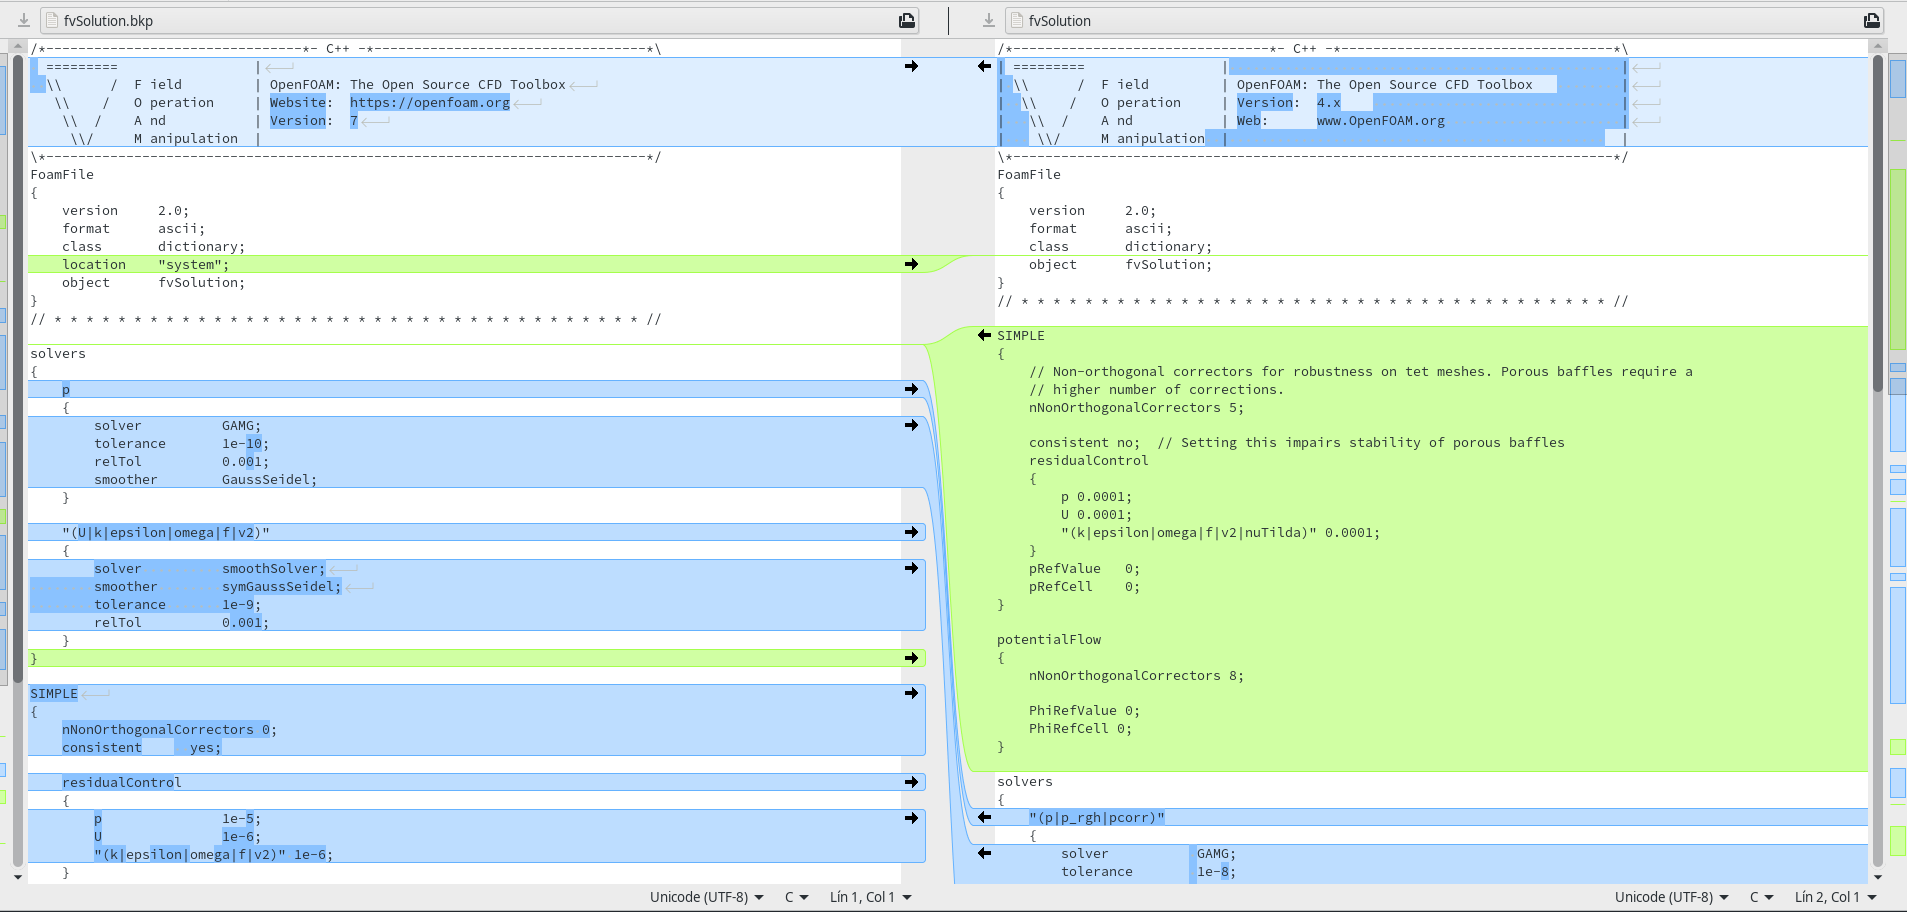
\includegraphics[width=0.8\textwidth]{Figuras/03_MELD.png}}
		 \caption{Comparación archivos fvSolution.bkp (izquierda) con fvSolution (derecha)} \label{fg:meld}
\end{figure*}

Volviendo a FreeCAD, podremos ejecutar la simulación con \textit{RUN}. Observar que la evolución de los residuales (figura \ref{fg:03_sf_residuales}) comienza a oscilar sobre un valor aproximadamente constante a partir de la iteración número 1000 sin llegar nunca a las tolerancias definidas en \textit{system/fvSolution}. 

\begin{figure*}[htb]
	%\centerline{
		%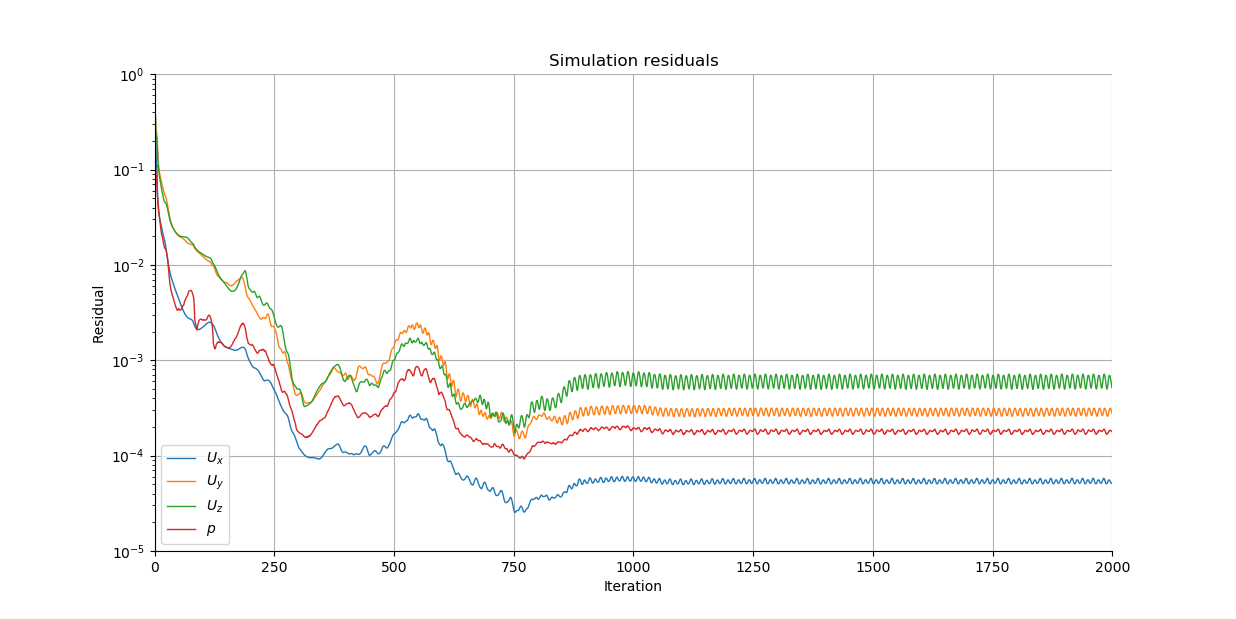
\includegraphics[width=0.8\textwidth]{Figuras/03_SF_RESIDUALES.png}}
	\caption{Evolución de residuales con simpleFoam} \label{fg:03_sf_residuales}
\end{figure*}

Sin necesidad de esperar a que termine de correr la simulación, podemos ver la evolución del perfil en ParaView. En la figura \ref{fg:03_sf_U} se muestra el campo de velocidades para una iteración bastante avanzada de la simulación (1700). Al comparar con pasos de tiempo consecutivos, no se aprecian grandes diferencias en los campos de velocidad o presión, por lo que asumiremos que la simulación fue satisfactoria.
FreeCAD descompone el caso en varios procesadores, por lo que para ver los resultados en ParaView debemos seleccionar "DecomposedCase".

\begin{figure*}[htb]
	%\centerline{
		%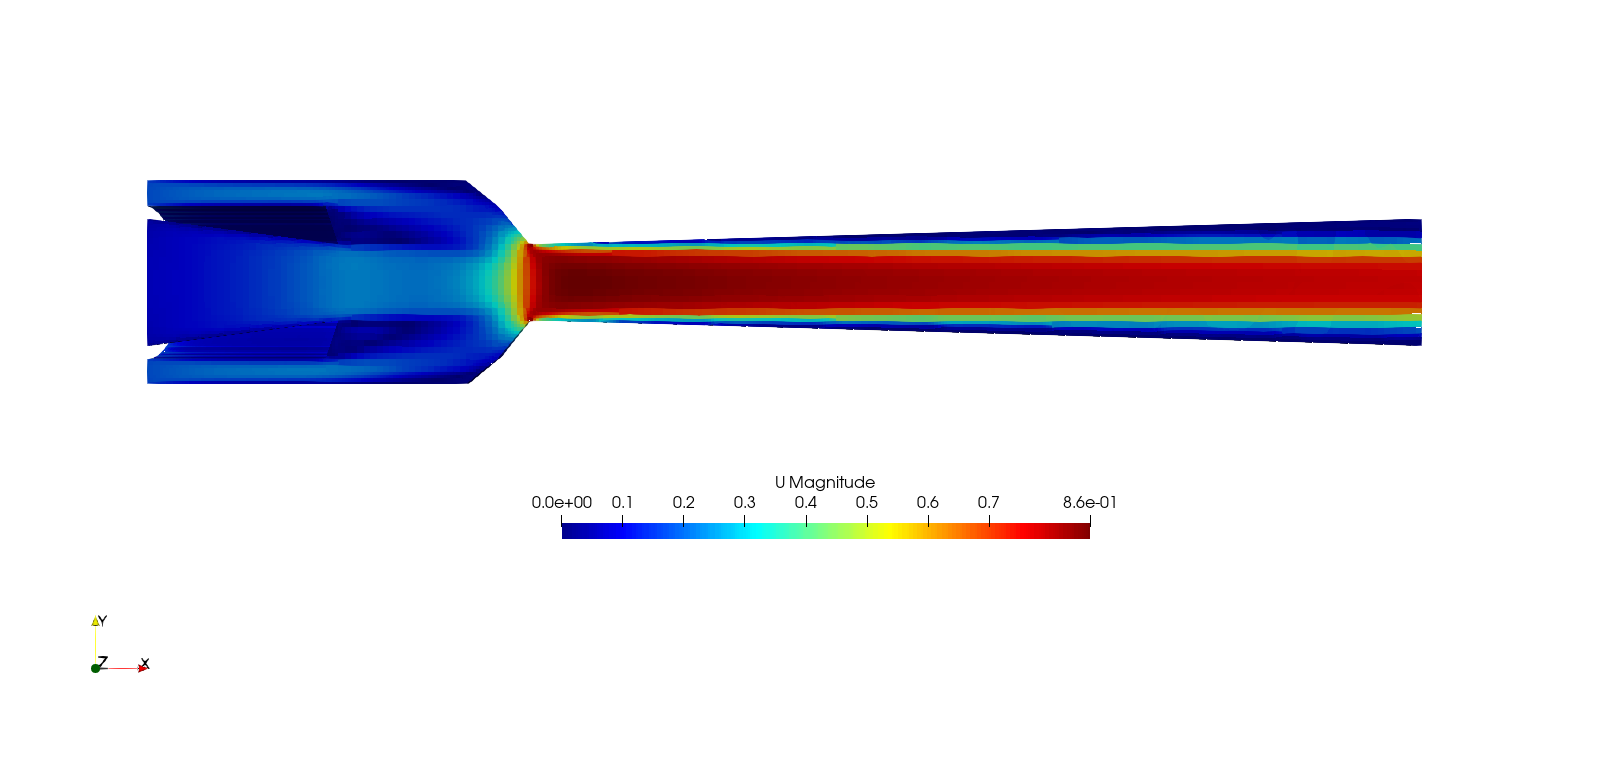
\includegraphics[width=0.8\textwidth]{Figuras/03_SF_U.png}}
	\caption{Campo de velocidad U obtenido} \label{fg:03_sf_U}
\end{figure*}

\subsection{Reconstrucción del caso}
Ya sabemos de los informes anteriores que necesitamos copiar el campo de presión y velocidad obtenidos con esta simulación en otro directorio que contenga el caso de la simulación RTD. Como el caso fue ejecutado en varios procesadores, en el directorio principal no encontraremos los pasos de simulación. Éstos se encuentran en las carpetas \texttt{processor*} y los archivos están divididos (caso descompuesto).

Para reconstruir el caso debemos ejecutar el comando \texttt{\$ reconstructPar} en el directorio \textit{case}. Ahora encontraremos los campos de presión y velocidad para la iteración 2000 en el directorio principal.

\section{SIMULACIÓN SCALARTRANSPORTFOAM}

Preparamos el caso de transporte escalar copiando la malla en \texttt{meshCase/constant/polyMesh} en el directorio \texttt{constant} del caso \texttt{RTD}. También traeremos de la simulación de \textit{simpleFoam} el campo de velocidad \texttt{2000/U} al directorio de condiciones iniciales \texttt{0/U} en \texttt{RTD}.
Ajustamos las condiciones en \texttt{system} según los valores del \href{https://github.com/guillerolle/casos_cfd/blob/master/03/RTD/system}{repositorio}

\subsection{Descomposición en varios procesadores}
En el diccionario \href{https://github.com/guillerolle/casos_cfd/blob/master/03/RTD/system/decomposeParDict}{system/decomposeParDict} se indica la cantidad de subprocesos que se usarán para correr la simulación. Ajustar este valor en función de la cpu dónde se ejecuta. En este caso, se utilizarán 4 procesadores.

Ejecutamos \texttt{\$ createPatch -overwrite} y luego \texttt{\$ decomposePar -force} en el directorio principal y aparecerán ahora directorios \texttt{processor*}. Ahora, con el siguiente comando podremos iniciar la simulación: \par 
\texttt{\$ mpirun -n 4 scalarTransportFoam -parallel | \\} 
\texttt{>  tee log.scalarTransportFoam}

En la figura \ref{fg:04_stf_res} se ven los residuales de esta simulación. Recordando que es una simulación en estado transitorio, se puede concluir que el solver llega a una solución constante a partir del 1er segundo de simulación aproximadamente.

\begin{figure*}[htb]
	%\centerline{
		%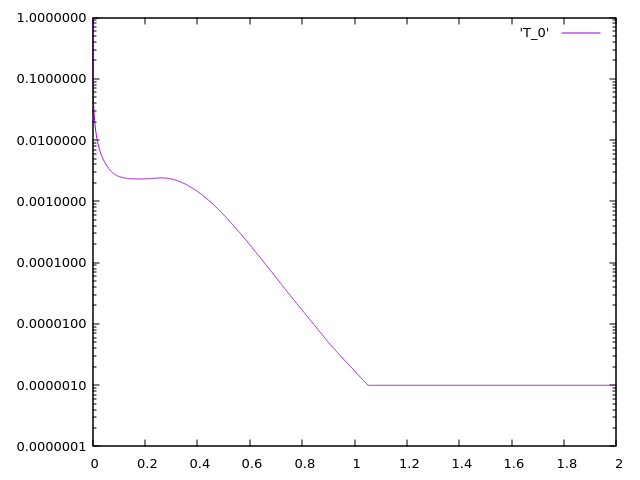
\includegraphics[width=0.8\textwidth]{Figuras/04_STF_RESIDUAL_T.png}}
	\caption{Evolución de residuales con simpleFoam} \label{fg:04_stf_res}
\end{figure*}

\section{POST-PROCESO}

Vamos a usar principalmente \textit{ParaView} para analizar los resultados. En la figura \ref{fg:05_stream_t} podemos ver unas líneas de traza coloreadas en función de la concentración de agroquímico. Se hizo la muestra sobre una línea paralela al eje 'Y' para facilitar la interpretación del campo tridimensional. Se observa que la mayor parte del mezclado se realiza, en realidad, justo después de la cámara de mezclado. Este fenómeno se puede adjudicar a que el flujo es laminar (por el modelo propuesto en la simulación), dificultando el mezclado dentro de la cámara.

\begin{figure*}[htb]
	%\centerline{
		%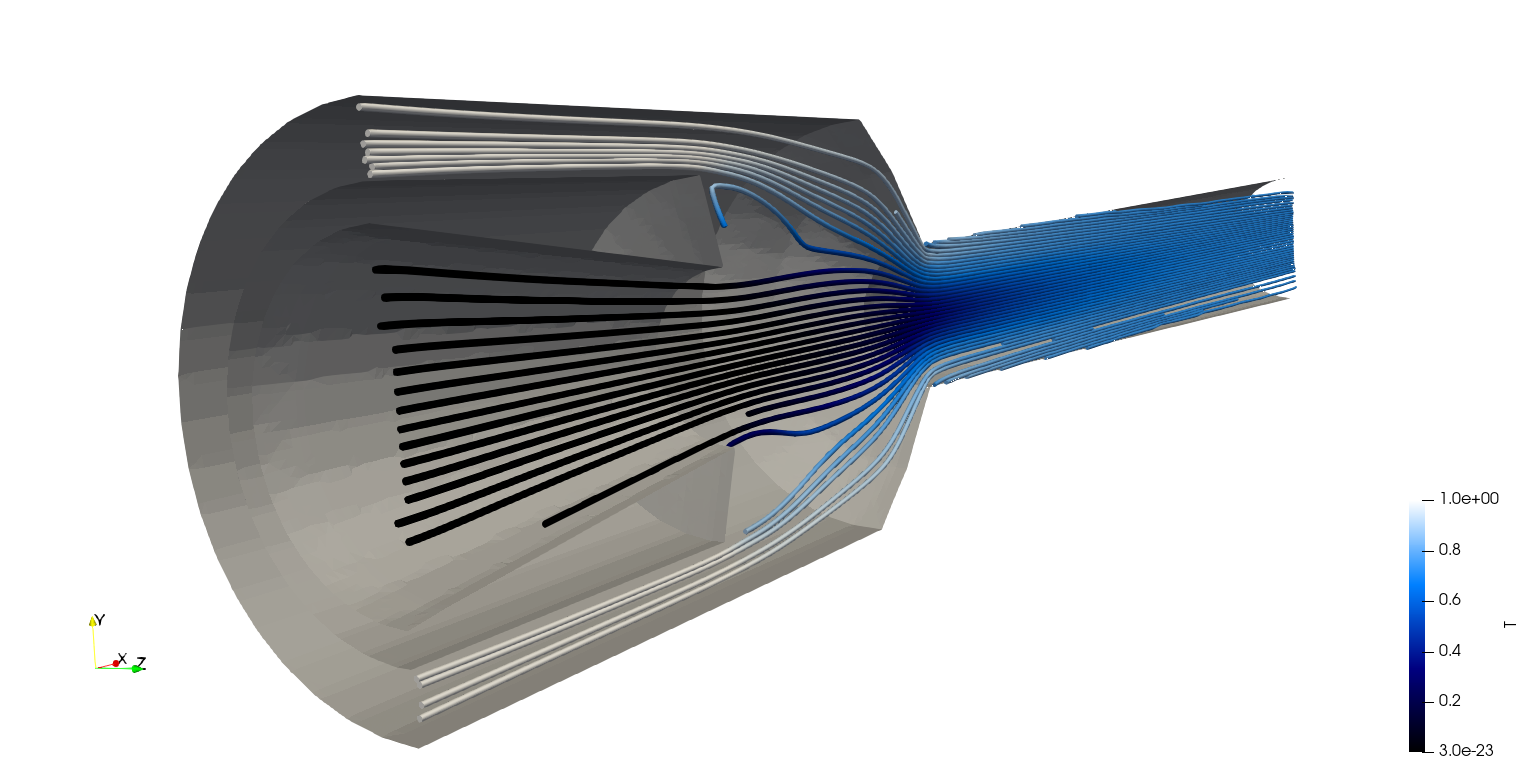
\includegraphics[width=0.8\textwidth]{Figuras/05_STREAMLINES_T.png}}
	\caption{Líneas de traza coloreadas según concentración de agroquímico} \label{fg:05_stream_t}
\end{figure*}

Con una rápida inspección visual parece ser que a la salida la concentración de agroquímico es aproximadamente 0.7. Usando la función de posproceso definida en el caso de OpenFOAM como \textit{patchAverage} calculamos la evolución de la concentración en la superficie de salida. El valor final es de 72\%. En la figura \ref{fg:05_avg_T} se muestra esta evolución.


\begin{figure*}[htb]
	\centerline{
		  %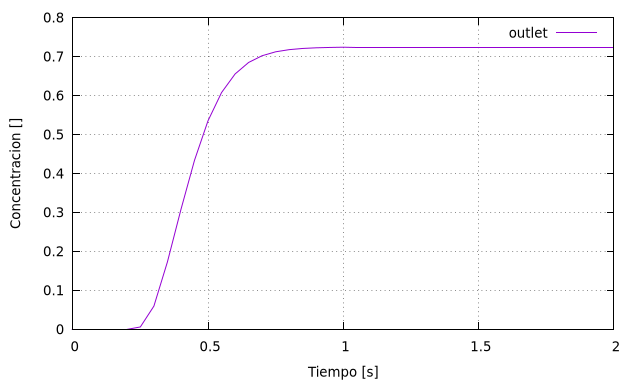
\includegraphics[width=0.6\textwidth]{Figuras/05_AVERAGE_T.png}
	}
	\caption{Evolución la concentración en la salida del dispositivo} \label{fg:05_avg_T}
\end{figure*}

Si hacemos varios cortes en distintas secciones del dispositivo podemos ver cómo varía la distribución de concentración en el eje 'X', como se muestra en la figura \ref{fg:05_STR_XY}. Observar que el agroquímico no llega a difundir perfectamente en la salida (color verde).


\begin{figure*}[htb]
	\centerline{
		  %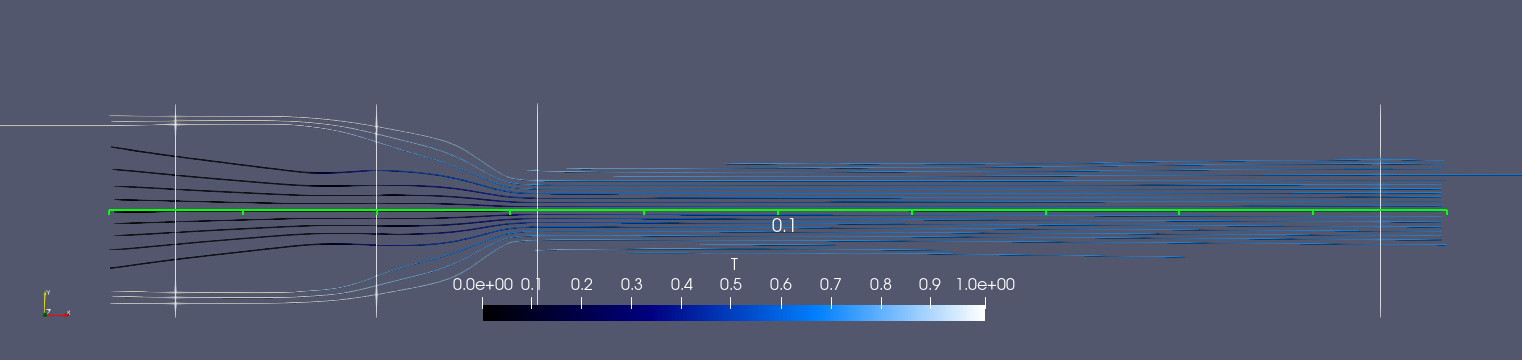
\includegraphics[width=0.8\textwidth]{Figuras/05_STREAM_DIVISIONES.png}
	}
	\centerline{
		  %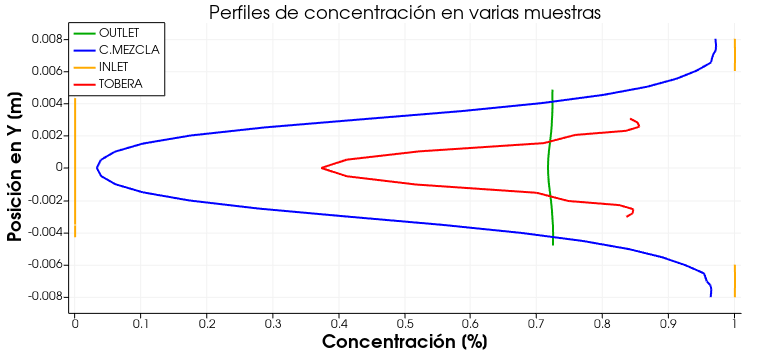
\includegraphics[width=0.8\textwidth]{Figuras/05_T_VARIAS.png}
	}
	\caption{Distribución de concentración de agroquímico en varias secciones del dispositivo} \label{fg:05_STR_XY}
\end{figure*}

Sería conveniente analizar más detalladamente la concentración en la superficie de salida del dispositivo. Si bien debería mantener una simetría respecto del eje del dispositivo, en la figura  \ref{fg:05_outlet} queda en evidencia que esto no sucede así. Una posible razón de este inconveniente, es la malla ortogonal alineada con los ejes cartesianos en todo el volumen de la muestra. 

\begin{figure*}[htb]
	\centerline{
		  %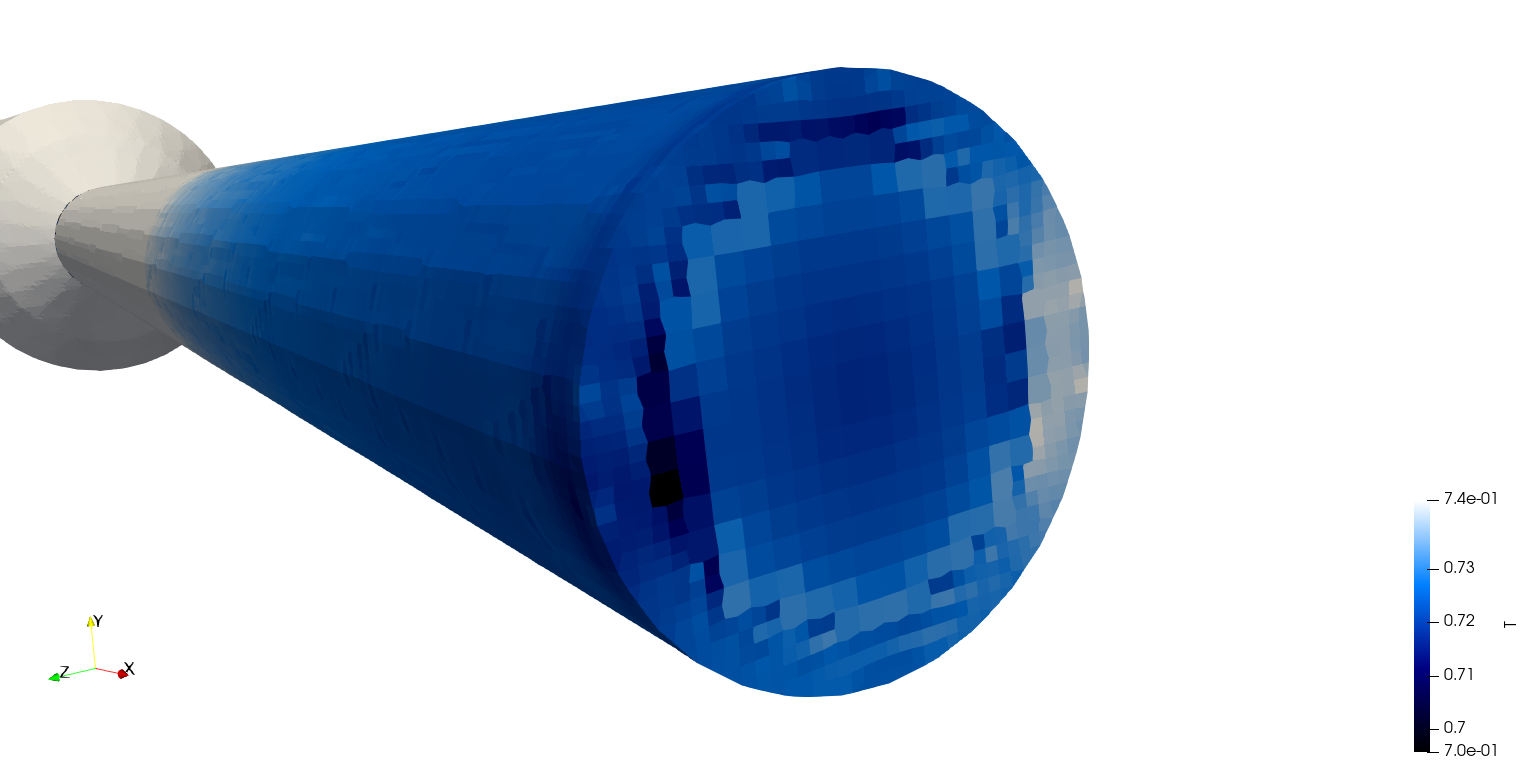
\includegraphics[width=0.8\textwidth]{Figuras/05_OUTLET_T.png}
	}
	\caption{Concentración en Outlet. Valores por celda} \label{fg:05_outlet}
\end{figure*}

Esto puede implicar errores en la interpolación entre celdas. Será diferente para celdas contenidas en el plano XY (que debería tener componentes de velocidad únicamente en X e Y) que una que esté girada a 45 grados respecto a un plano paralelo al YZ. En este caso, el método debería interpolar en dirección a vértices de las celdas hexahedrícas y no sobre caras o aristas, generando diferencias entre celdas de una misma sección. En la figura \ref{fg:05_hexa_glyph} se muestra esta idea.


\begin{figure*}[htb]
	\centerline{
		  %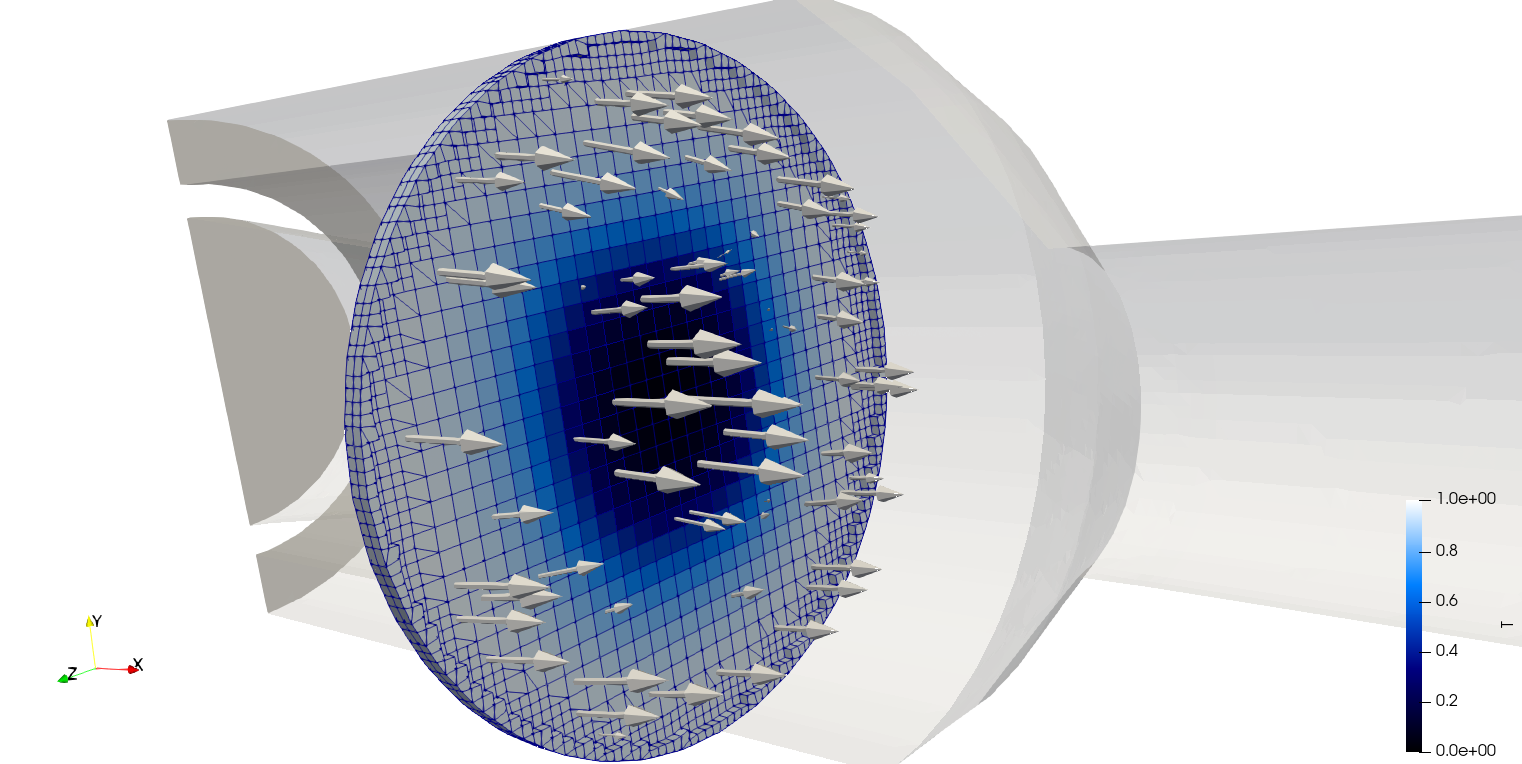
\includegraphics[width=0.8\textwidth]{Figuras/05_GLYPH_HEXA.png}
	}
	\caption{Malla ortogonal en un caso simétrico respecto a un eje} \label{fg:05_hexa_glyph}
\end{figure*}

Además, hay que tener en cuenta que el método no pudo reducir los residuales por más de $10^{-4}$, generando estas discrepancias con lo esperado. En ciertos casos, estas diferencias pueden ser perfectamente aceptables mientras que en otros no. Esto es criterio del ejecutante y de las exigencias que debe cumplir la simulación.

\section{CONCLUSIONES}
En este informe preparamos y ejecutamos el primer caso tridimensional del dispositivo. Generamos una malla sobre un modelo arbitrario creado en \textit{FreeCAD} y ejecutamos las simulaciones correspondientes. Surgieron dificultades con la convergencia de las simulaciones, mostrando de alguna manera la influencia del mallado sobre los resultados.

Además, se hace notar que los resultados esperados en cuanto a la concentración promedio en el outlet debería ser similar a los del \href{https://github.com/guillerolle/informes_cfd/blob/master/Informe02.pdf}{informe anterior} (34\%) pero en este caso dio valores muy diferentes (72\%). Revisando las condiciones impuestas, los valores de presión en los inlets debía ser de 300 kPa, pero por error se hicieron las simulaciones con 0.3 kPa. No se realiza la simulación nuevamente ya que éstos valores generan mayores inconvenientes en la convergencia (con los mismos diccionarios en \texttt{system} los residuales no bajan de $10^{-2}$) y se considera un trabajo innecesario para los fines prácticos de este informe y adscripción. Se prefiere continuar con una simulación más avanzada en el siguiente informe.

Aprovechando que las condiciones de la simulación no permiten resolver adecuadamente el caso en estado estacionario, el siguiente informe se va a realizar utilizando un solver transitorio \href{https://www.openfoam.com/documentation/guides/latest/doc/guide-applications-solvers-incompressible-pimpleFoam.html}{pimpleFoam}.

%\section*{AGRADECIMIENTOS} Los autores agradecen a ...
% ACKNOWLEDGEMENTS FOR FULL ARTICLES
%
%\bibliography{amcapaper}
\end{document}
